%\documentclass[14pt]{beamer}
\documentclass{beamer}

\usetheme{Copenhagen}
% \usetheme{Boadilla}
% \usecolortheme{beaver}
\setbeamercolor{alerted text}{fg=orange}
\setbeamercolor{background canvas}{bg=white}
\setbeamercolor{block body alerted}{bg=normal text.bg!90!black}
\setbeamercolor{block body}{bg=normal text.bg!90!black}
\setbeamercolor{block body example}{bg=normal text.bg!90!black}
\setbeamercolor{block title alerted}{use={normal text,alerted text},fg=alerted text.fg!75!normal text.fg,bg=normal text.bg!75!black}
\setbeamercolor{block title}{bg=blue}
\setbeamercolor{block title example}{use={normal text,example text},fg=example text.fg!75!normal text.fg,bg=normal text.bg!75!black}
\setbeamercolor{fine separation line}{}
\setbeamercolor{frametitle}{fg=white}
\setbeamercolor{item projected}{fg=white}
\setbeamercolor{normal text}{bg=white,fg=black}
\setbeamercolor{palette sidebar primary}{use=normal text,fg=normal text.fg}
\setbeamercolor{palette sidebar quaternary}{use=structure,fg=structure.fg}
\setbeamercolor{palette sidebar secondary}{use=structure,fg=structure.fg}
\setbeamercolor{palette sidebar tertiary}{use=normal text,fg=normal text.fg}
\setbeamercolor{section in sidebar}{fg=brown}
\setbeamercolor{section in sidebar shaded}{fg=grey}
\setbeamercolor{separation line}{}
\setbeamercolor{sidebar}{bg=red}
\setbeamercolor{sidebar}{parent=palette primary}
\setbeamercolor{structure}{bg=black, fg=white!30!blue!60!green}
\setbeamercolor{subsection in sidebar}{fg=brown}
\setbeamercolor{subsection in sidebar shaded}{fg=grey}
\setbeamercolor{title}{fg=white}
\setbeamercolor{titlelike}{fg=white}

% Szép kék
% \setbeamercolor{structure}{bg=black, fg=white!10!green!40!blue}

\frenchspacing

% Language packages
\usepackage[utf8]{inputenc}
\usepackage[T1]{fontenc}
\usepackage[magyar]{babel}

% AMS
\usepackage{amssymb,amsmath}

% Graphic packages
\usepackage{graphicx}

% Syntax highlighting
\usepackage{listings}

\usepackage{tikz}

%\begin{figure}[htb]
%\begin{center}
%	\includegraphics[scale=0.4]{ps_times.png}
%\end{center}
%\end{figure}

\usefonttheme{professionalfonts} % using non standard fonts for beamer
\usefonttheme{serif} % default family is serif
\usepackage{tgbonum}

% ==============
\begin{document}
% ==============

\title[Strukturált adatok kinyerése PDF dokumentumokból]{Strukturált adatok kinyerése PDF dokumentumokból}
\author[Molnár Fanni]{\textbf{Molnár Fanni}}
\institute[]{Miskolci Egyetem}
\date{2020. június 23.}

% --------------------
\frame{\titlepage}

% --------------------
\begin{frame}[fragile]
\frametitle{Bevezetés}

A dokumentumaink egy jelentős része elektronikus formában érhető el. Ennek közkedvelt formátuma a PDF (Portable Document Format).
A dolgozat olyan módszereket mutat be, amelyek a képek strukturális elemeit ismerik fel.

\smallskip

Az elemzésnek két fő alternatívája lehet:

\bigskip

\begin{itemize}
    \item PDF API-k használatával lehet kinyerni a fájlokból a dokumentum adatait
    \item PDF képpé alakítása, majd képfeldolgozási módszerekkel való elemzése
\end{itemize}

\end{frame}

% --------------------
\begin{frame}[fragile]
\frametitle{Dokumentum szerkezete}

A dokumentumok szerkezete lehet nagyon egyszerű, de igen komplikált is.

\smallskip

\begin{figure}[!tbp]
  \centering
  \begin{minipage}[b]{0.45\textwidth}
    
\includegraphics[width=\textwidth]{images/page_simple.png}
  \end{minipage}
  \hfill
  \begin{minipage}[b]{0.45\textwidth}
    
\includegraphics[width=\textwidth]{images/page_complicated.png}
  \end{minipage}
\end{figure}

\end{frame}

% --------------------
\begin{frame}[fragile]
\frametitle{Dokumentum felbontása}

A felbontásokhoz a dokumentumban levő, összefüggő fehér területeket kerestem (margó, sorköz stb.). Meghatároztam az átlagos intenzitást a dokumentum minden sorára és oszlopára majd ezek mentén kezdtem meg a felbontást.

\end{frame}

% --------------------
\begin{frame}[fragile]
\frametitle{Dokumentum felbontása}

\begin{figure}[!tbp]
  \centering
  \begin{minipage}[b]{0.6\textwidth}
    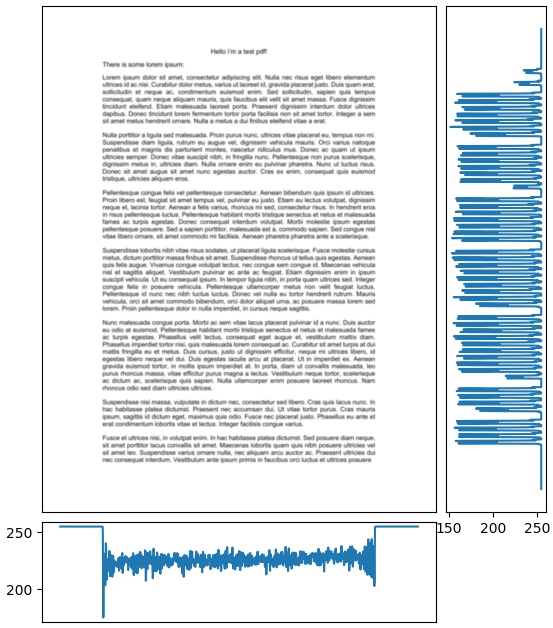
\includegraphics[width=\textwidth]{images/intensity.png}
  \end{minipage}
\end{figure}

\end{frame}

% --------------------
\begin{frame}[fragile]
\frametitle{Margók}

A margók levágásához az intenzitásokat tartalmazó tömb elejétől indultam el, majd addig haladtam amíg fehér, egybefüggő területet találtam.

\bigskip

A kapott margók nélküli dokumentumot fogom tovább bontani paragrafusokra, sorokra, szavakra majd karakterekre.

\end{frame}

% --------------------
\begin{frame}[fragile]
\frametitle{Paragrafusok és sorok}

A paragrafusokra bontásnál azt feltételezem hogy a térköz nagyobb mint a sorköz.

\bigskip

A soroknál ugyan azon algoritmussal dolgoztam mint a paragrafusoknál, annyi különbséggel hogy itt a küszöbérték az sokkal alacsonyabb volt.

\end{frame}

% --------------------
\begin{frame}[fragile]
\frametitle{Paragrafusok és sorok}

\begin{figure}[!tbp]
  \centering
  \begin{minipage}[b]{1\textwidth}
    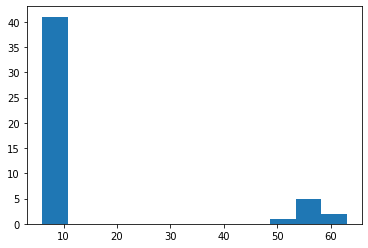
\includegraphics[width=\textwidth]{images/segment_hist.png}
  \end{minipage}
\end{figure}

\end{frame}

% --------------------
\begin{frame}[fragile]
\frametitle{Szavak}

A szavakra és karakterekre bontást már nem az y, hanem az x tengely mentén végeztem.

\bigskip

A már kivágott sorokat felhasználva kerestem a fehér területeket, tapasztalati érték alapján legalább 5 darabot, majd egyenként lementettem a megtalált szavakat.

\end{frame}

% --------------------
\begin{frame}[fragile]
\frametitle{Karakterek}

A szavak betűkre bontása már egy érdekesebb témakör. Ennél az algoritmusnál már nem a világos, hanem épp hogy a sötét részeket kerestem, és ha már 1 pixelnek megfelelő sötét részt is találtam már mentettem az adott indexet.

\begin{figure}[!tbp]
  \centering
  \begin{minipage}[b]{0.45\textwidth}
    
\includegraphics[width=\textwidth]{images/ligatura.png}
  \end{minipage}
\end{figure}

\end{frame}

% --------------------
\begin{frame}[fragile]
\frametitle{Bonyolultabb dokumentum felbontása}

\begin{figure}[!tbp]
  \centering
  \begin{minipage}[b]{0.3\textwidth}
    
\includegraphics[width=\textwidth]{images/page_complicated.png}
  \end{minipage}
  \hfill
  \begin{minipage}[b]{0.3\textwidth}
    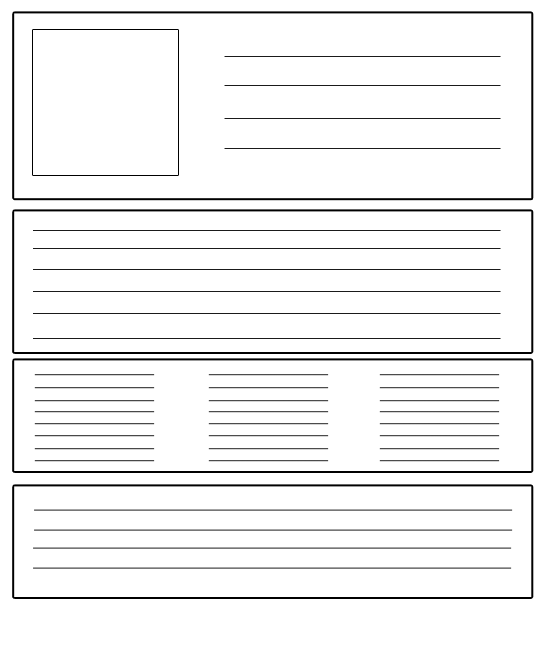
\includegraphics[width=\textwidth]{images/page_complicated2.png}
  \end{minipage}
  \hfill
  \begin{minipage}[b]{0.3\textwidth}
    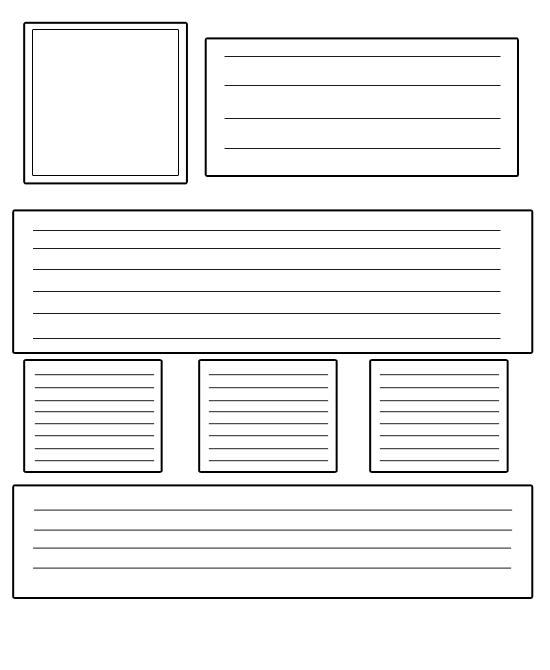
\includegraphics[width=\textwidth]{images/page_complicated3.png}
  \end{minipage}
\end{figure}

\end{frame}

% --------------------
\begin{frame}[fragile]
\frametitle{Képek és szövegek megkülönböztetése}

\begin{figure}[!tbp]
  \centering
  \begin{minipage}[b]{1\textwidth}
    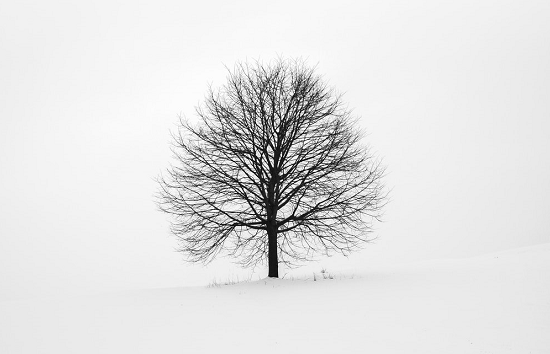
\includegraphics[width=\textwidth]{images/tree.png}
  \end{minipage}
\end{figure}

\end{frame}

% --------------------
\begin{frame}[fragile]
\frametitle{Képfelismerés neurális háló segítségével}

A képfelismerés javításának érdekében a Python-ban megtalálható Keras nevezetű neurális háló API-val kezdtem el foglalkozni.

\begin{figure}[!tbp]
  \centering
  \begin{minipage}[b]{0.48\textwidth}
    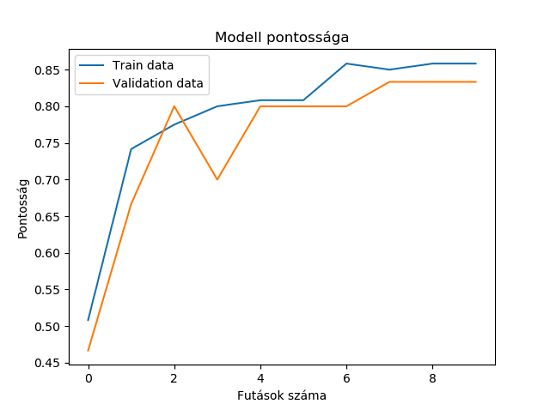
\includegraphics[width=\textwidth]{images/accuracy.png}
  \end{minipage}
  \hfill
  \begin{minipage}[b]{0.48\textwidth}
    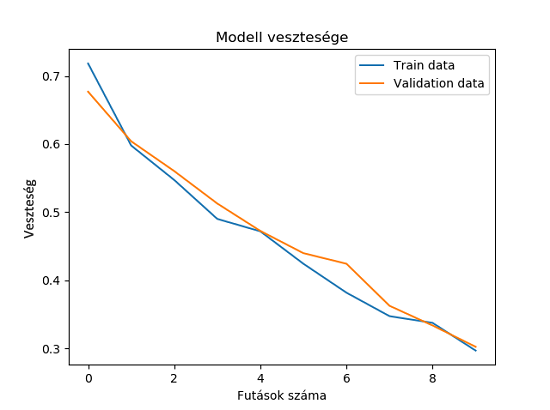
\includegraphics[width=\textwidth]{images/loss.png}
  \end{minipage}
\end{figure}

\end{frame}

% --------------------
\begin{frame}[fragile]
\frametitle{A vizsgálatokhoz készített programok}

\begin{itemize}
    \item Python programozási nyelv (NumPy, OpenCV, Matplotlib függvénykönyvtárak)
    \item Jupyter munkafüzetek
    \item Tesseract, Keras függvénykönyvtárak
\end{itemize}

\end{frame}

% --------------------
\begin{frame}[fragile]
\frametitle{Képek vágása és további feldolgozása}

A first\_try nevű Python modul fogja össze az alábbi modulokat:

\bigskip

\begin{itemize}
    \item crop\_methods
    \item get\_methods
    \item manage\_directories
\end{itemize}

\end{frame}

% --------------------
\begin{frame}[fragile]
\frametitle{Jupyter munkafüzetek használata}

A módszerek kutatásának, a kapott eredmények elemzésének egy másik módját a Jupyter munkafüzetek használata jelenti.

\bigskip

\begin{itemize}
    \item page\_structure.ipynb
    \item partitioning.ipynb
    \item blob\_shapes
\end{itemize}

\bigskip

Megfelelő futásukhoz szükségesek a következő függvénykönyvtárak: NumPy, OpenCV, Matplotlib és pdf2image.

\end{frame}

% --------------------
\begin{frame}[fragile]
\frametitle{Összegzés}

\begin{itemize}
    \item A szerkezeti elemzés bizonyos dokumentumok esetében nagyon bonyolult
    \item A felvetett problémára csak akkor lehetne tökéletes megoldást adni, hogy ha pontosan definiálva lenne, hogy milyen elemek és hogyan fordulhatnak elő egy dokumentumban
\end{itemize}

\end{frame}

% --------------------
\begin{frame}[fragile]
\frametitle{Hivatkozott irodalmak}

\begin{itemize}
    \item Gary Bradski and Adrian Kaehler. Learning OpenCV: Computer vision with the OpenCV library. " O’Reilly Media, Inc.", 2008.
    \item Vaibhaw Singh Chandel. Deep learning based text recognition (ocr) using tesseract and opencv. www.learnopencv.com, 2018.
    \item Antonio Gulli and Sujit Pal. Deep learning with Keras. Packt Publishing Ltd, 2017.
    \item Python Package Index. pdf2image. https://pypi.org/project/pdf2image/, 2020.
    \item Project Jupyter. Jupyter. https://jupyter.org, 2020.
\end{itemize}

\end{frame}

% --------------------
\begin{frame}[fragile]
\frametitle{\ }

\begin{center}

    \Large

    \textbf{Köszönöm szépen a figyelmet!}

    \bigskip

\end{center}

\end{frame}

\end{document}

